\documentclass{beamer}


\usepackage[utf8]{inputenc}
\usepackage{pgfpages}
\usepackage{xcolor}

\setbeameroption{show notes}
\setbeamertemplate{note page}[plain]
\setbeameroption{show notes on second screen=left}

\usetheme{Warsaw}
\graphicspath{ {./images/}{../images/}{../kcov-swedencpp/images/}{../../kcov-swedencpp/images/}{output/} }

\title[What's in a binary?] %optional
{What's in a binary?}

%\subtitle{A short story}

\author{Simon Kågström}

\institute
{
  Consultant\\
  \texttt{https://github.com/SimonKagstrom/emilpro}
}

%\logo{\includegraphics[height=1.5cm]{lion-logo.png}}

\begin{document}

\begin{frame}
  \titlepage
  \note{
    My name is Simon Kågström and I work as a consultant, currently at Profoto. Tonight I will present
    emilpro, which is a graphical disassembler.
  }
\end{frame}

\begin{frame}{Background}
  \begin{itemize}
    \item I have a few themes that I often return to in my projects
    \item One of these is disassembly
  \end{itemize}
  \note{
    I don't know about you, but at least I tend to return to a few themes over and over again.
    These projects are never finished, and rarely really working, but they are fun to work on.

    For some of these, I've done multiple reimplementations, and the topic of this talk is one
    of them. This is actually the third implementation, the first one was started almost 20 years ago
    now as a Python application called Dissy. You get a sense of how old I am now, I guess!

    That one really just parsed objdump output, so after a few years I thought I could do better,
    and rewrite it in C++ and use libraries for the parsing instead. So a bit over 10 years ago, I
    rewrote it as "emilpro", which is a pun on IDA pro which at least then was the state of the art.

    It was sort of working, but bitrotted and a few years later it wasn't even possible to compile
    anymore. But when I again needed disassembly this year, I thought I'd just rewrite it again
    and that's the topic of this talk. The third implementation now, and counting!
  }
\end{frame}


\begin{frame}
  \frametitle{Demo}
  \note{
    I'll start with a small demo of the application.
  }

  
\includegraphics[width=\linewidth]{kalkyl}
  % Start the app. Show symbols, filtering, cross-reference, jump lanes, address history
\end{frame}

\begin{frame}
  \frametitle{Outline}
    \begin{itemize}
      \item Part I: Motivation
      \item Part II: What does the disassembly writer need?
      \item Part III: Why is this easier now than 10 years ago?
    \end{itemize}
  \end{frame}

\begin{frame}{Part I: Motivation}
  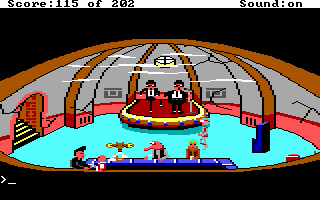
\includegraphics[width=8cm]{sq1_blues_brothers}
\end{frame}

\begin{frame}[fragile]{Motivation}
  \begin{itemize}
    \item C/C++ with inline assembly
    \item Systems and programming environments where a debugger wasn't available
  \end{itemize}
  \begin{Example}
    \begin{semiverbatim}
      \scriptsize
\#define \_syscall1(type,name,atype,a) type name(atype a) \{
        unsigned long out;
        \_\_asm\_\_ volatile (
        ".set  push\\n.set  noreorder\\n"
        ".short 0xfefe\\n"
        ".short \%1\\n"
        ".pushsection .cibylstrtab, \\"aS\\"\\n"
        "1: .asciz \\"" \#name "\\"\\n"
        ".popsection\\n"
        ".long 1b\\n"
        ".set\\tpop\\n"
        "move \%[out], \$2\\n
        : [out]"=d" (out)
        : "r"(a)
        : "memory", "\$2"
        );
        return (type) out;
\}
    \end{semiverbatim}
  \end{Example}

  \note{
    I've during my career, although mostly for non-work related tasks, multiple times had to rely on
    diassembly for debugging and understanding how things work while working on low-level stuff.

    Back in the days, I was also writing a lot of inline assembly, and side effects of that is easy
    to get almost correct, so that it breaks in subtle ways when more complex code is used. If you've
    used GCC inline assembly, you'll know that it's quite powerful but it's very important to correctly
    specify input, output correct, as well as side-effects, which are known as clobbered. I had to
    look the word up by the way, and clobbered means "to hit someone or something hard and repeatedly".
    That summarizes GCC inline assembly well, I think!

    In some instances, I had no way of debugging the code, but could get backtraces and register dumps.
    The disassembly was then the only way to figure out what was going on.
  }
\end{frame}

\begin{frame}{Backstory}
  \begin{itemize}
    \item Objdump output is cumbersome to navigate through
    \item I wanted a graphical application that allows easier navigation
  \end{itemize}
  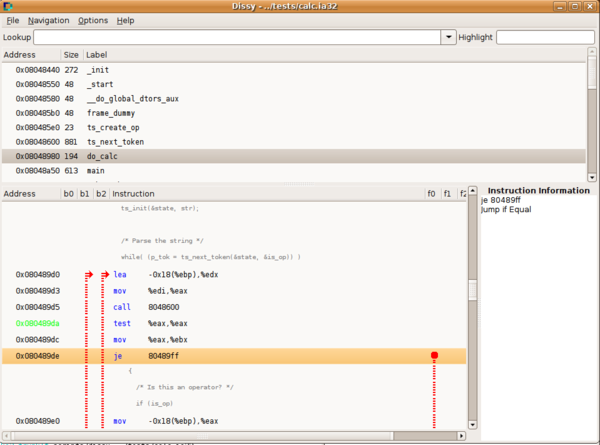
\includegraphics[width=4.5cm]{dissy-with-instruction-box-600}
  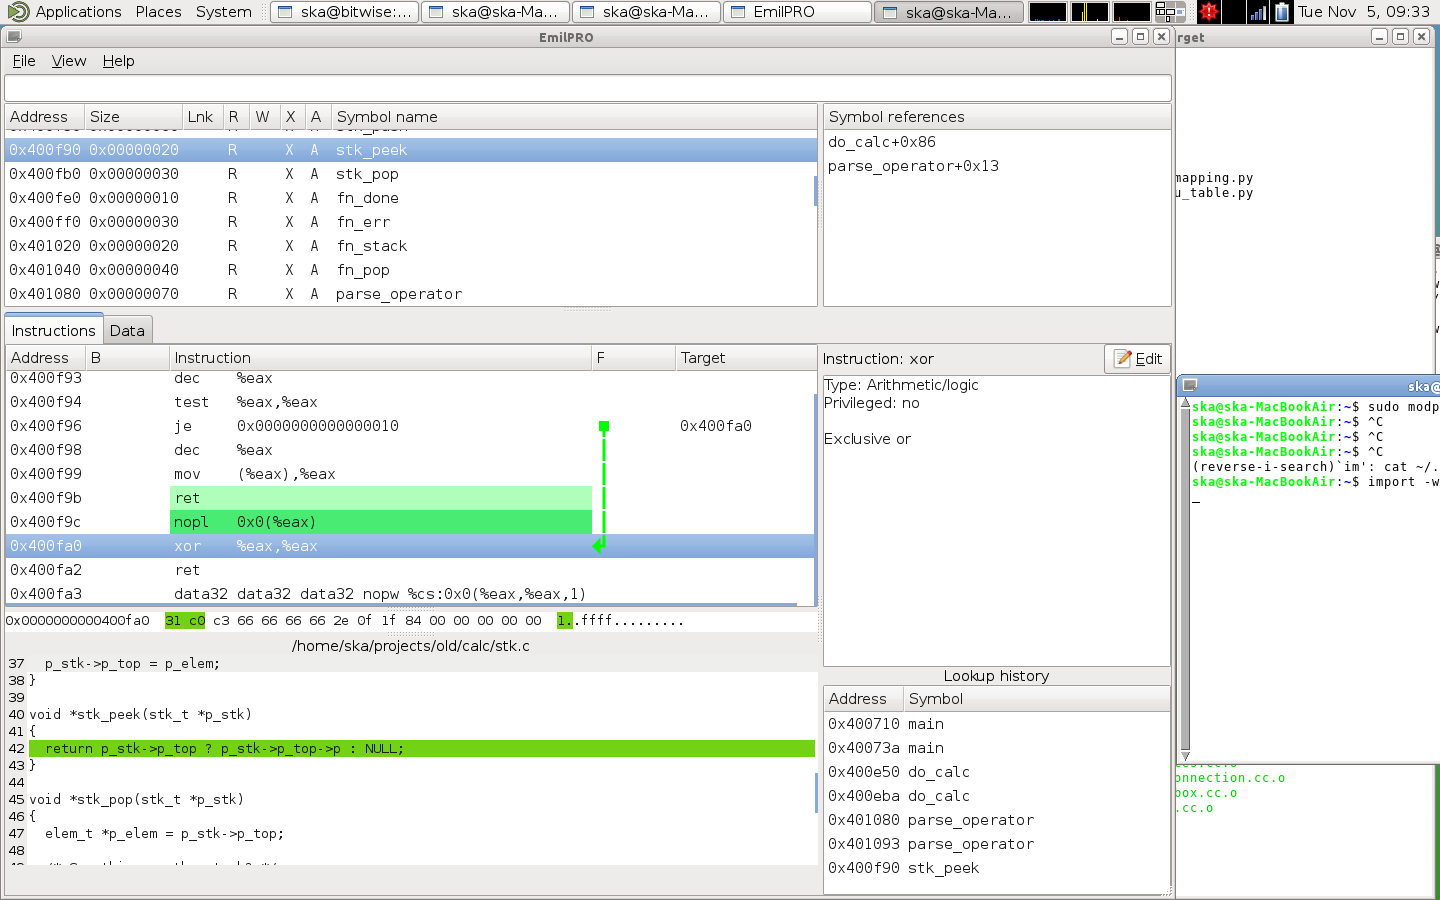
\includegraphics[width=6cm]{old_emilpro}
  \note{
  Using plain Objdump for this is very cumbersome, so I wanted an easier way to navigate the
  disassembly.

  So in 2006, I wrote a small python application called Dissy. It was a simple graphical frontend
  to objdump and nm, and simply parsed the text output from those tools. It was good enough for my
  purposes, but it was too slow for larger binaries.

  Around 2011-2012, I was working on the Linux kernel in my day job, which was impossible to use
  with dissy. I therefore thought I'd rewrite it in C++, via libbfd instead of parsing objdump
  output. The binutils libbfd, as in binary file descriptor, is the base of objdump anyway, so why not
  use it directly?

  That's the image on the right, and I called it EmilPRO as a pun on IDA pro. I got something working,
  but for reasons I'll get back into, it bitrot and a few years ago it was impossible to even compile.
  About a year ago, I stumbled upon another question to which the answer was disassembly (namely: How
  can this short C++ snippet compile to 14KB!?), and I thought I'd try to revive it. It turned out to
  be a more or less complete rewrite, and that's the topic of the rest of the talk.
}
\end{frame}

\begin{frame}{Part II: What is needed for a disassembler?}
  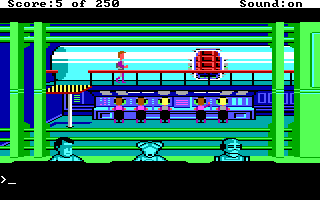
\includegraphics[width=8cm]{sq2_computer_room}
\end{frame}

\begin{frame}{Binary formats}
  \begin{itemize}
    \item \textbf{Linux/FreeBSD} etc: ELF
    \item \textbf{MacOS}: Mach-O
    \item \textbf{Windows}: PE
  \end{itemize}
    % ELF + DWARF
    % Mach-O
    % PE
    % The three rules for an instruction set architect
    \note{
      The binary format is used for executables and linkable object files. These are the
      three probably most commonly used formats today.

      ELF is used for Linux, FreeBSD and others, but also as an intermediate format for a
      lot of embedded systems. MacOS uses the Mach-O format, from the Mach microkernel. You'll
      notice here that the binary format engineers have a sense of humor, and you also have
      the DWARF debugging format to go with ELF and also Mach-O. If you invent a new format,
      I'd suggest ORC as a name.

      The execption to the funniness is Windows, which simply calls their format pee.

      For MS-DOS, there were multiple formats, COM, MZ and NE.
    }
  \end{frame}


\begin{frame}{How to write a dissassembler?}
  \begin{columns}
    \begin{column}{0.5\textwidth}
      I did not write everything from scratch!

      \begin{itemize}
        \item \textbf{libbfd}: Part of binutils, used for reading binary files
        \item \textbf{capstone}: Disassembler library
        \item \textbf{Qt}: GUI framework
      \end{itemize}
    \end{column}
    \begin{column}{0.5\textwidth}
      \includegraphics[width=5cm]{emilpro_structure}
    \end{column}
  \end{columns}
  \note{
    I didn't write everything from scratch.

    It's like Newton said: "If I hadn't been standing on the shoulders of giants, I wouldn't have reached
    the apple."

    The three main building stones are Qt, the GUI framework, libbfd and capstone. libbfd reads binary files
    to gather symbols, relocations and instruction data which the disassembler then picks up. The sectiond
    data, for text sections are then fed to capstone, which disassembles it into instructions.
  }
\end{frame}

\begin{frame}{Loading a binary}
  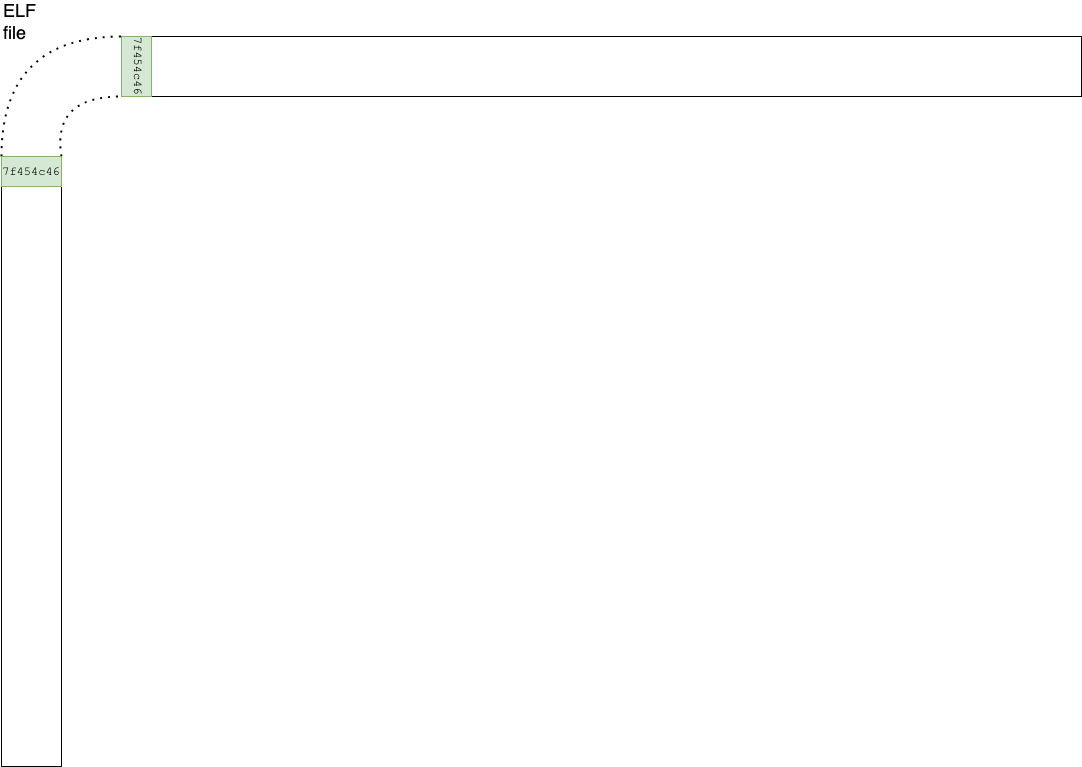
\includegraphics[width=8cm]{elf_background}
  \note{
    So let's say you have a file with the ELF magic. How do you go about to get the instructions 
    out of it? The vertical and horizontal views are both of the same file, but I use the vertical one
    to illustrate the raw data in the file, and the horizontal to display data structures.

    Basic ELF is actually fairly simple to write a parser for. However, the devil is in the
    details, but libbfd helps a lot with that.
  }
\end{frame}

\begin{frame}{Loading a binary, sections}
  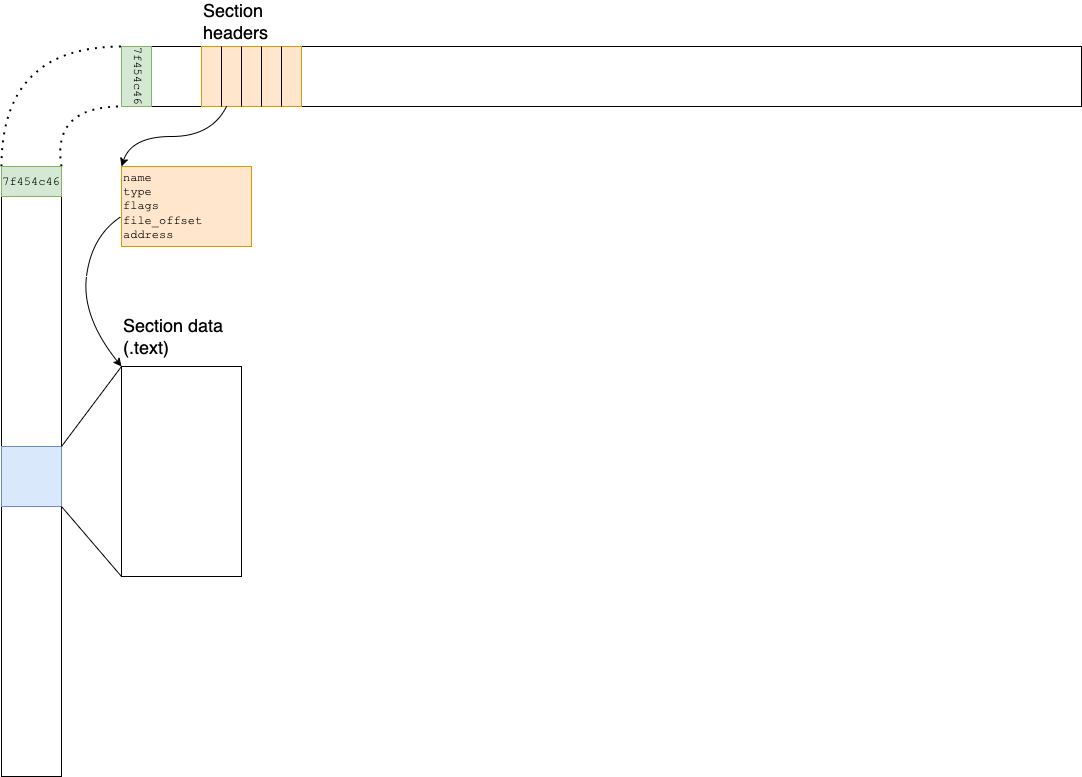
\includegraphics[width=8cm]{elf_sections}

  \note{
    The sections are the basic building blocks of the ELF file, and similar concepts are also present for
    other binary formats. It's the first thing we need to find our instructions, and if that was the only
    goal we could basically stop here.

    The ELF file contains section headers, which can be used to find where the actual section data is in
    the file, i.e., at which file offset the section data begins. It also contains a name, via the string
    table, and some flags to indicate what type of section it is.

    Not all sections are loaded into memory (e.g., debug information), but for those that are, the memory
    address of the section is also present. These days, a lot of code is position-independent, so that
    might not be relevant.

    So, although we could just read the data we just found (indicated via the blue box) and disassemble
    it, it would only give us raw instructions with little less information. Another problem with this is that
    it's easy to get lost among the instructions, since the compiler might mix data and instructions so that
    the disassembler starts disassembling in the middle of instructions. Especially on x86.
  }
\end{frame}

\begin{frame}{Loading a binary, symbols}
  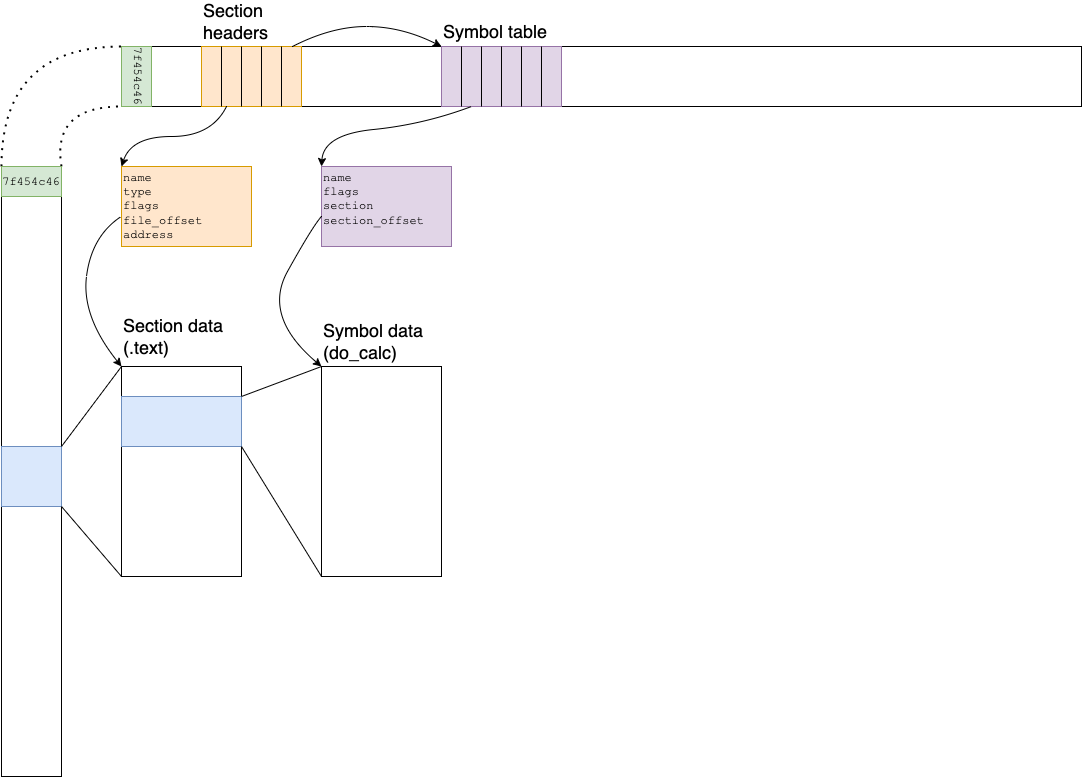
\includegraphics[width=8cm]{elf_symbols}
  \note{
    So in addition to the section data, we really want and need symbol information as well. At least for
    this type of disassembler, where the focus is debugging and understanding the code, there's no way
    around it. Symbols can be found in their own section, called the symbol table. It's shown on the
    horizontal view, with a pointer to it from the section table.

    Each symbol contains information about the symbol type, e.g., function, data object, or even a
    section. For functions and data, it also has information about visibility, i.e., local to the
    object file or globally visible. There's also a name, and a reference to the section the symbol
    belongs to. This, together with the section offset tells us where the instructions for the
    symbol resides, which is illustrated on the image.

    There's also a size for the symbol, but this is actually optional and can't be relied upon.
    Therefore, to get the chunks to disassemble, I simply order the symbols via a std::map, and
    disassemble everything from one symbol to the next. The last is terminated by the section end.

    So, with this, we're finally able to get the disassembled instructions.
  }
\end{frame}

\begin{frame}{Loading a binary, instructions}
  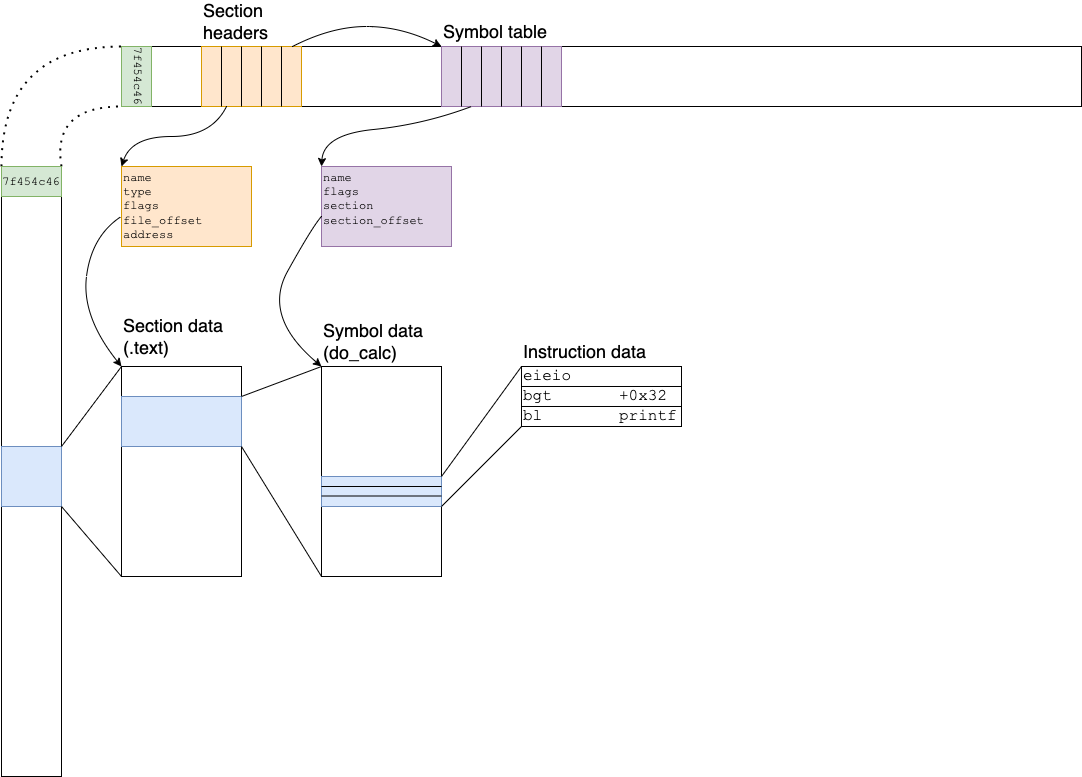
\includegraphics[width=8cm]{elf_instructions}

\note{
  So here, you see how three instructions are disassembled. The disassembly has been done by capstone,
  which also provides some metadata about the instructions. In particular, it's used here to determine
  which instructions are branches (or jumps), and where they jump to. That's used to generate the
  "jump lanes" in the disassembly view.

  Jumps and branches are typically local to the symbol, but calls to functions are not. They are
  handled in mostly the same way, but the target address needs to be looked up from the symbol table.
  Finally, capstone also has information about used registers, which the disassembler uses to highlight
  registers in different colors in the disassembly view.

  And by now, you'd think we would be done and ready for beer, but there's one more problem. There's
  a call to printf here, and where's printf located? Let's say this is an object file, and printf
  resides in another file or library, that the linker resolves.
}

\end{frame}

\begin{frame}{Loading a binary, relocations}
  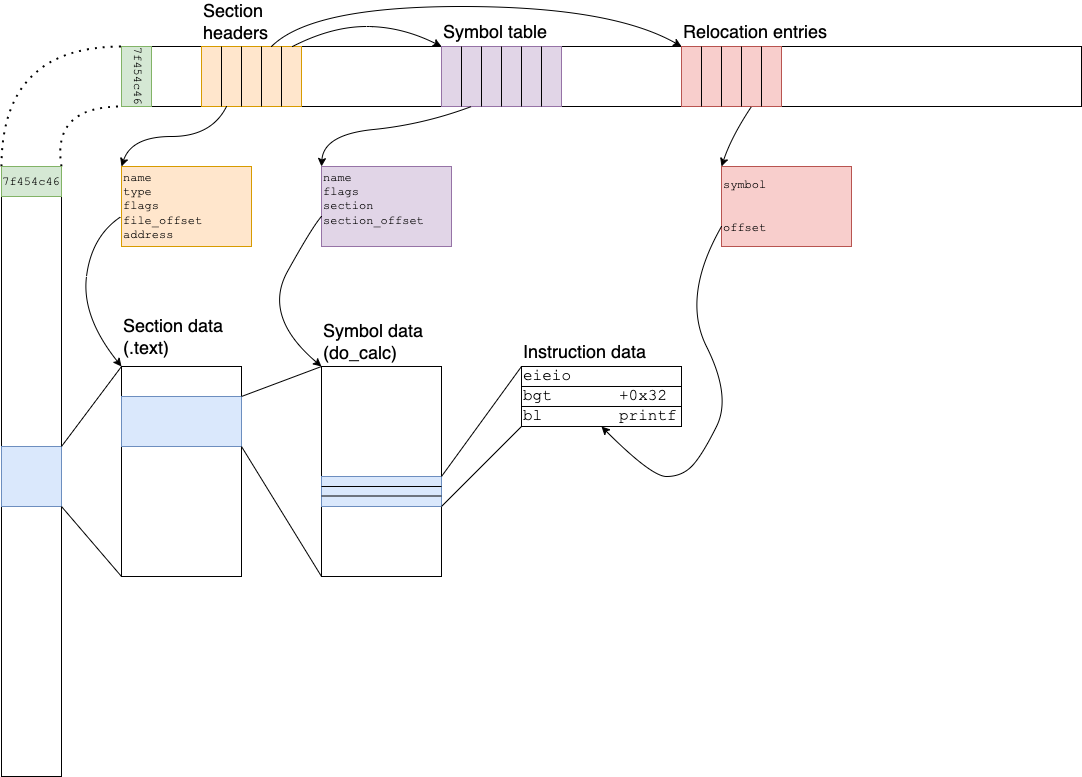
\includegraphics[width=8cm]{elf_relocations}

  \note{
  So to resolve printf, a relocation entry has been added. The purpose of the relocation entry in this
  case is for the linker to resolve it to to a correct address, and patch the instruction with the
  resolved address. Depending on the architecture, there might be multiple relocations pointing to the
  same target, for example with fixed-size instruction sets where a full address might not fit in one
  instruction.

  It's interesting to read the libbfd documentation about relocations by the way. It's quite informative,
  but also a bit archaic. They use the Motorola 68000 instruction set for the first relocation example.
  How many here have used the 68000? The next example is then the COFF format on the Motorola 88000,
  which at least I haven't used.

  Anyway, why is the disassembler interested in relocations? Well, in this case, the call instruction
  doesn't really say anything, since the compiler doesn't know where printf is. With the relocation,
  the disassembler can resolve the call to printf. But where does it end up?
}
\end{frame}

\begin{frame}{Loading a binary, relocations}
  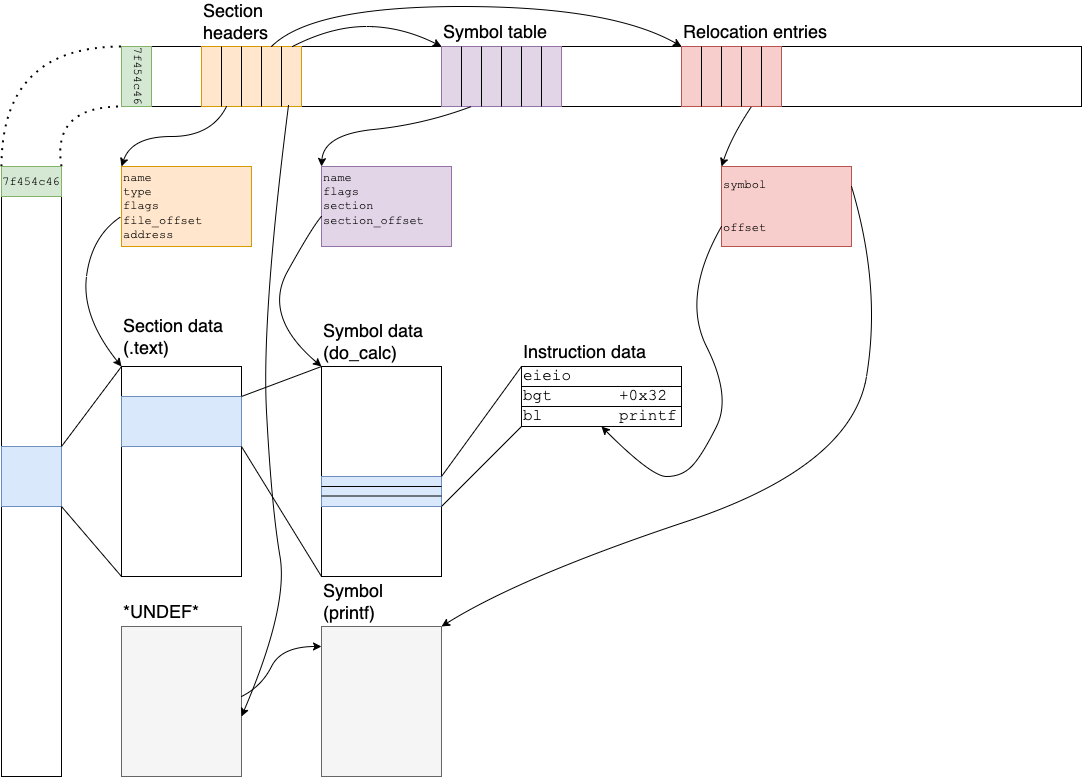
\includegraphics[width=8cm]{elf_undefined_section}
  \note{
  The final piece of the puzzle is then handled by a special section for undefined symbols. Here, the
  relocation entry points to the printf symbol, which in it's symbol header has a reference to the
  undefined section. For the disassembler, this is really only used to mark the symbol as gray in the
  symbol view. For the instruction view, the relocation entry is enough to resolve the call to printf.

  % Check if the section is actually present in an ELF file

  Now, in a linked executabe, there are usually also undefined symbols and relocations, where shared
  libraries are used. I will not go into that here, but there are some additional aspects to consider
  there. One thing is that resolving for example each call to printf would be quite expensive, if it's
  called in many places. Therefore, an indirection is often used, so that the call is done into the PLT
  or Procedure Linking Table. Then, the relocation only needs to be done in the PLT, and this can also
  be lazily, the first time a particular function is called.
  }
\end{frame}

\begin{frame}{Part III: Why is this easier now than 10 years ago?}
  %move from binutils
  %c++11+
  %conan
  %copilot
\end{frame}

\begin{frame}{Bad design decisions in the original project}
  \begin{itemize}
    \item<1-> feature creep: core functionality sketchy, work on irrelevant features
    \item<2> libbfd for disassembly: the multiarch-dev issue
  \end{itemize}

  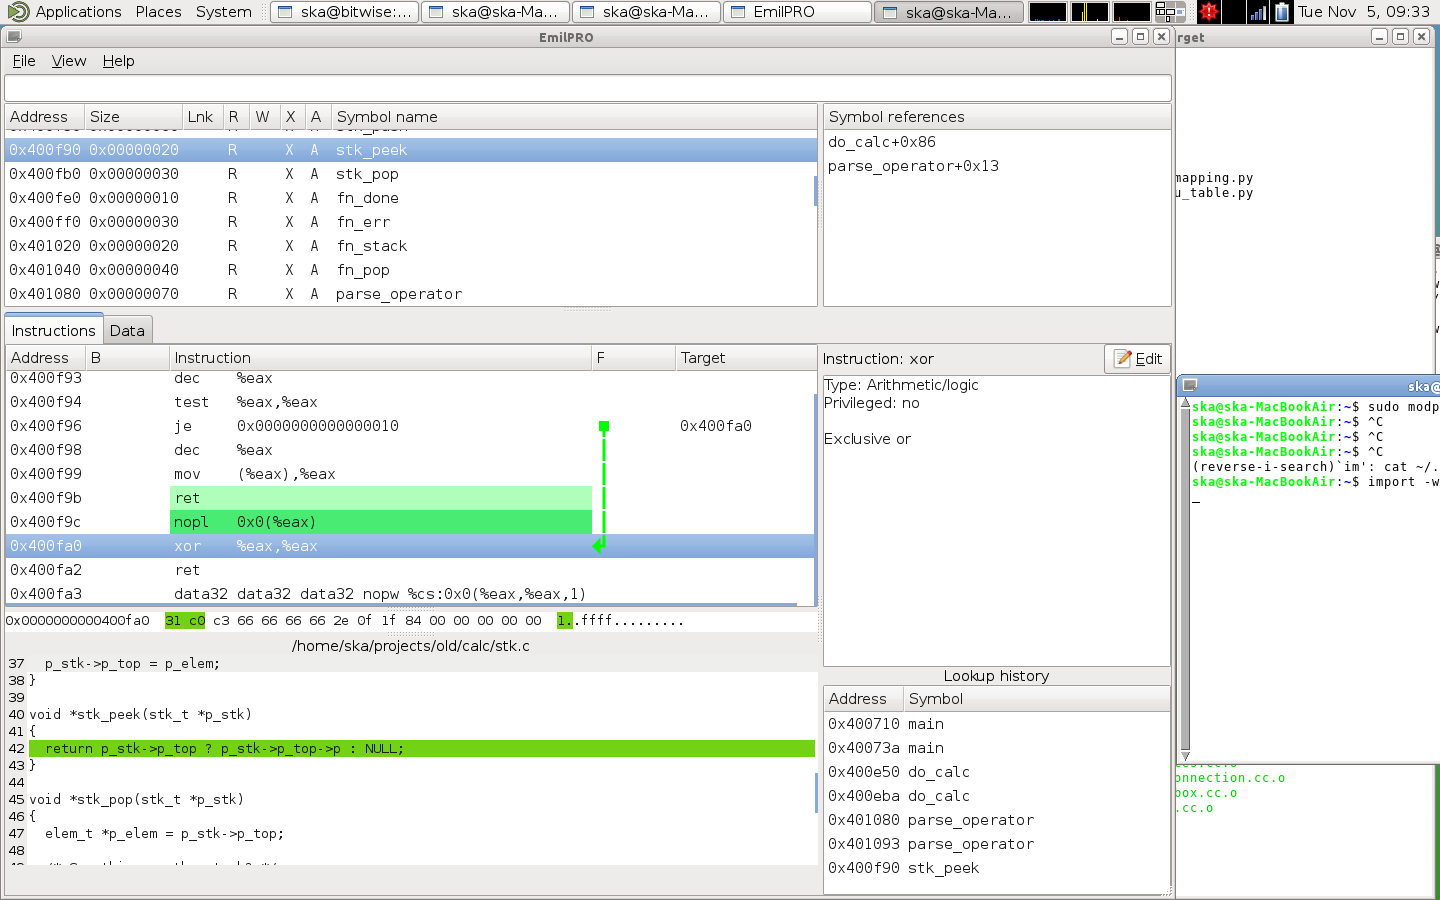
\includegraphics[width=8cm]{old_emilpro}

  \note<1>{
  The first mistake I did with the original project was the feature scope. I had lots of ideas, for example
  being able to edit instructions, which would then be pushed to a web service to share with other users.
  That was quite a bit of work, while at the same time core features like resizing the window didn't work
  well.

  Of course, I did this on my spare time, and basically did what I found interesting. Window resizing
  and learning Qt creator wasn't something I really longed to do. But the end result was that the
  project had features which were useless, while the usability of what you really wanted was so-so.
  }
  \note<2>{
  But the main reason I failed had to do with libbfd. There are actually two parts to this. The first
  is that even though the documentation is quite good, there are parts of it which are rather difficult
  to understand. In particular, this goes for relocations. Since I had recently worked with ELF
  relocations in another project, I simply picked up the raw ELF relocation types from the section
  file offset and used them. This made it ELF-only, and pretty much Linux-only.

  The second is that I decided to use libbfd as a diassembler as well. This sort of makes sense, since
  it's the C3PO of binary parsers and can handle 6 million forms of instruction sets. However, if you
  want to disassemble something other than the host architecture, you'll need the multiarch build of it.
  Unfortunately, the development package isn't for the multiarch build, so I resorted to build it by
  myself as part of the build process, for a fixed binutils version.

  Apart from prolonging the build time by an hour the first time, this also meant that a few years
  ahead, it was impossible to build emilpro because of kernel and libc changes. So for the new
  version, I swore to never use anything other than the distiribution package for libbfd, no self-
  builds!
  }

  % built my own binutils. Bitrot and was unbuildable later
\end{frame}

\begin{frame}[fragile]{C++20 and onwards}
  \begin{itemize}
    \item The previous implementation was done just around the C++11 introduction, but used C++03
    \item Now C++23, so much better!

    \begin{block}{C++03}
      \begin{semiverbatim}
        \scriptsize
for (InstructionList\_t::const\_iterator it = instructions.begin();
     it != instructions.end();
     ++it) \{
      \end{semiverbatim}
    \end{block}
    \begin{block}{C++23}
      \begin{semiverbatim}
        \scriptsize
for (const auto& insn : m\_instructions)
\{
      \end{semiverbatim}
    \end{block}
  \end{itemize}

  \note{
    I started the previous version in 2012, and at least I was just starting to learn C++11. Therefore,
    it was mainly a C++03 project at the time. As probably all of you know, C++ is a completely different
    language now.

    So the new version uses C++23, and a lot of things are both much more compact, and also a lot simpler
    to implement. Apart from saving typing with auto, I also use a lot of std::span, which is a nice
    way to avoid exposing underlying data structures. Lambdas make some things much cleaner, such as
    reacting to Qt signals.
  }
\end{frame}

\begin{frame}[fragile]{C++ infrastructure}
  \begin{itemize}
    \item The conan package manager
    \item The addres sanitizer

    \begin{block}{Conan}
      \begin{semiverbatim}
        \scriptsize
[requires]
doctest/2.4.11
trompeloeil/48
fmt/11.0.2
capstone/5.0.1
etl/20.39.4
libiberty/9.1.0

[generators]
CMakeDeps
CMakeToolchain

[layout]
cmake_layout
      \end{semiverbatim}
    \end{block}
  \end{itemize}
  \note{
    The second area where things have improved is around the C++ infrastructure. As I said before,
    I refused to build my own binutils in this version, but use the distribution package.
    However, for other dependencies, I now in general use the conan package manager. It's a very
    nice way to ensure consistent builds across different platforms, and sometimes to get newer
    versions of libraries than the distribution has.

    As I use MacOS these days, conan also helped me with a very special issue. The libbfd version
    in Homebrew is actually incomplete, since it doesn't ship with libiberty, which is a GNU utility
    library (think linking with minus liberty). I felt hopelessness for a while when I realized this,
    since it would be quite difficult to build emilpro apart from on my own machine. However, I then
    found out that libiberty actually exists as a conan package, so simply adding that resolved
    this issue.

    Now, there have been many improvements to the C++ infrastructure since 2012, but one I've
    become very dependent on is the address sanitizer. I tend to always enable it for the debug
    builds and unit tests, and it's really nice to be able to catch leaks and overwrites early.

    The final reason might be a bit controversial, namely
  }
\end{frame}

\begin{frame}{AI}
  \begin{itemize}
    \item I use Github copilot
    \item Very helpful with Qt development
  \end{itemize}
  \includegraphics<2>[height=8cm]{copilot_calls_functions}
  % Unit test example (drawing, ugly)
  % LaTeX example (bad)
  % Qt example (good)
  %copilot

  \note<1>{
    AI. I'm using github copilot via vscode.  I'll actually show you a few examples, starting with one
    from the unit tests.

    Copilot also tried to help me with the presentation.
  }
  \note<2>{
    But this is how it is with AI systems: You pass a question into a black box, wait for it to churnk
    and then something comes out. What goes on inside is a mystery, maybe even to the creators.
    It's almost like you'd want a disassembler.
  }

\end{frame}



\begin{frame}{Questions and comments!}
  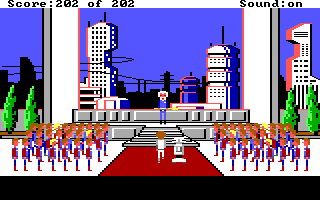
\includegraphics[width=\linewidth]{sq_final}

  Images from \url{http://www.falselogic.net/LetsPlay/SpaceQuest.html}

  Ian Lance Taylors linker series is the source of parts of this talk
  \url{https://www.airs.com/blog/index.php?s=Linkers}

  \note{
  First I have a teaser for my next talk. Do we have any people living or working in
  Uppsala here? Do you know that you live in the edge case?
  }
\end{frame}

\begin{frame}{Actors and objects}
  Actors
  \begin{itemize}
    \item \textbf{Compiler}
    \item \textbf{Linker}
    \item \textbf{Loader}
    \item \textbf{Disassembler}
  \end{itemize}
  Objects
  \begin{itemize}
    \item \textbf{Instructions}: The actual code
    \item \textbf{Sections}: Text, data, debug info etc
    \item \textbf{Symbols}: Functions/methods, variables, ...
    \item \textbf{Relocations}: Call sites for later resolving
  \end{itemize}
  % What is compiler, linker, loader?
  % Show in emilpro

  % Sections, symbols, relocations
  % Disassembler, compiler, linker, loader
\end{frame}



\begin{frame}{Producing a binary}
  \begin{columns}
    \begin{column}{0.5\textwidth}
      The compiler produces symbols, relocations plus data and text sections
    \end{column}
    \begin{column}{0.5\textwidth}
      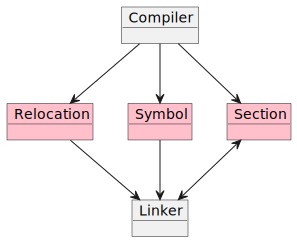
\includegraphics[width=5cm]{compiler_linker}
    \end{column}
  \end{columns}
  % Symbol example from ELF (dump reloc)
\end{frame}

\begin{frame}{Loading a binary}
  Different categories of binaries are handled differently:
  \begin{itemize}
    \item Execute from direct-mapped flash (embedded systems)
    \item Static executables
    \item Dynamic executables
    \item PIEs (Position-Independent Executables)
  \end{itemize}

  % Sections, symbols, relocations
  % Example from embedded system
  % Load sections into memory
  % Entry point
  % Disassembler, compiler, linker, loader
  \includegraphics[width=7cm]{loader}
\end{frame}

\begin{frame}{Static executables}

\end{frame}

\begin{frame}{Dynamic executables}
  % Global offset table (for global data, ignored here)
  % Procedure linkage table (for function calls)
  % Relocation entries are for the PLT, not the call sites
  % - when a function is called, it's called through the PLT
  % - the relocated PLT jumps to the function in the shared library
  % - at least Linux handles PLT resolving lazily, i.e., only when the
  %   function is called
\end{frame}

\begin{frame}{PIEs}
    % Relocation entries
    % Why are they needed?
\end{frame}

\begin{frame}{Relocations}
  \begin{itemize}
    \item If a non-local function is called, an undefined symbol is added
    \item The compiler adds a relocation entry for the call site
    \item When linking, the linker will resolve these symbols
    \item Different types depending on instruction
  \end{itemize}

  % Example from ELF (dump reloc)
\end{frame}

\begin{frame}{libbfd}
    %Example from documentation

    \note{
      libbfd is part of binutils, so is shipped with the linker.
    }
  \end{frame}


\end{document}
